% !TEX TS-program = xelatex
% !TEX encoding = UTF-8 Unicode

% GSET Summer 2023 - Tennessee Technological University
% Tristan Hill - June 06, 2023
% Turtorial 2 - Quadratic Equation

\documentclass[12pt]{article}

% Custom Preamble

\usepackage{../../py_tutorials}


% Title and Misc
\newcommand{\MNUM}{2} %Module Number
\newcommand{\MNAME}{Variables and Assignment} %Module Name
\newcommand{\TNAME}{The Quadratic Equation} %Tutorial Name
\pagestyle{myheadings}
\markright{{\large GSET - Introduction to Programming with Python}}

\begin{document}

\thispagestyle{plain}

\begin{center}
   {\bf \large GSET - Introduction to Programming with Python - Summer 2023} \vspace{5mm}\\
   {\bf \Large \MNAME \hspc -  Tutorial\hspc\MNUM\hspc - \TNAME}\vspace{3mm}\\
   
\end{center}

 \hspace*{3cm}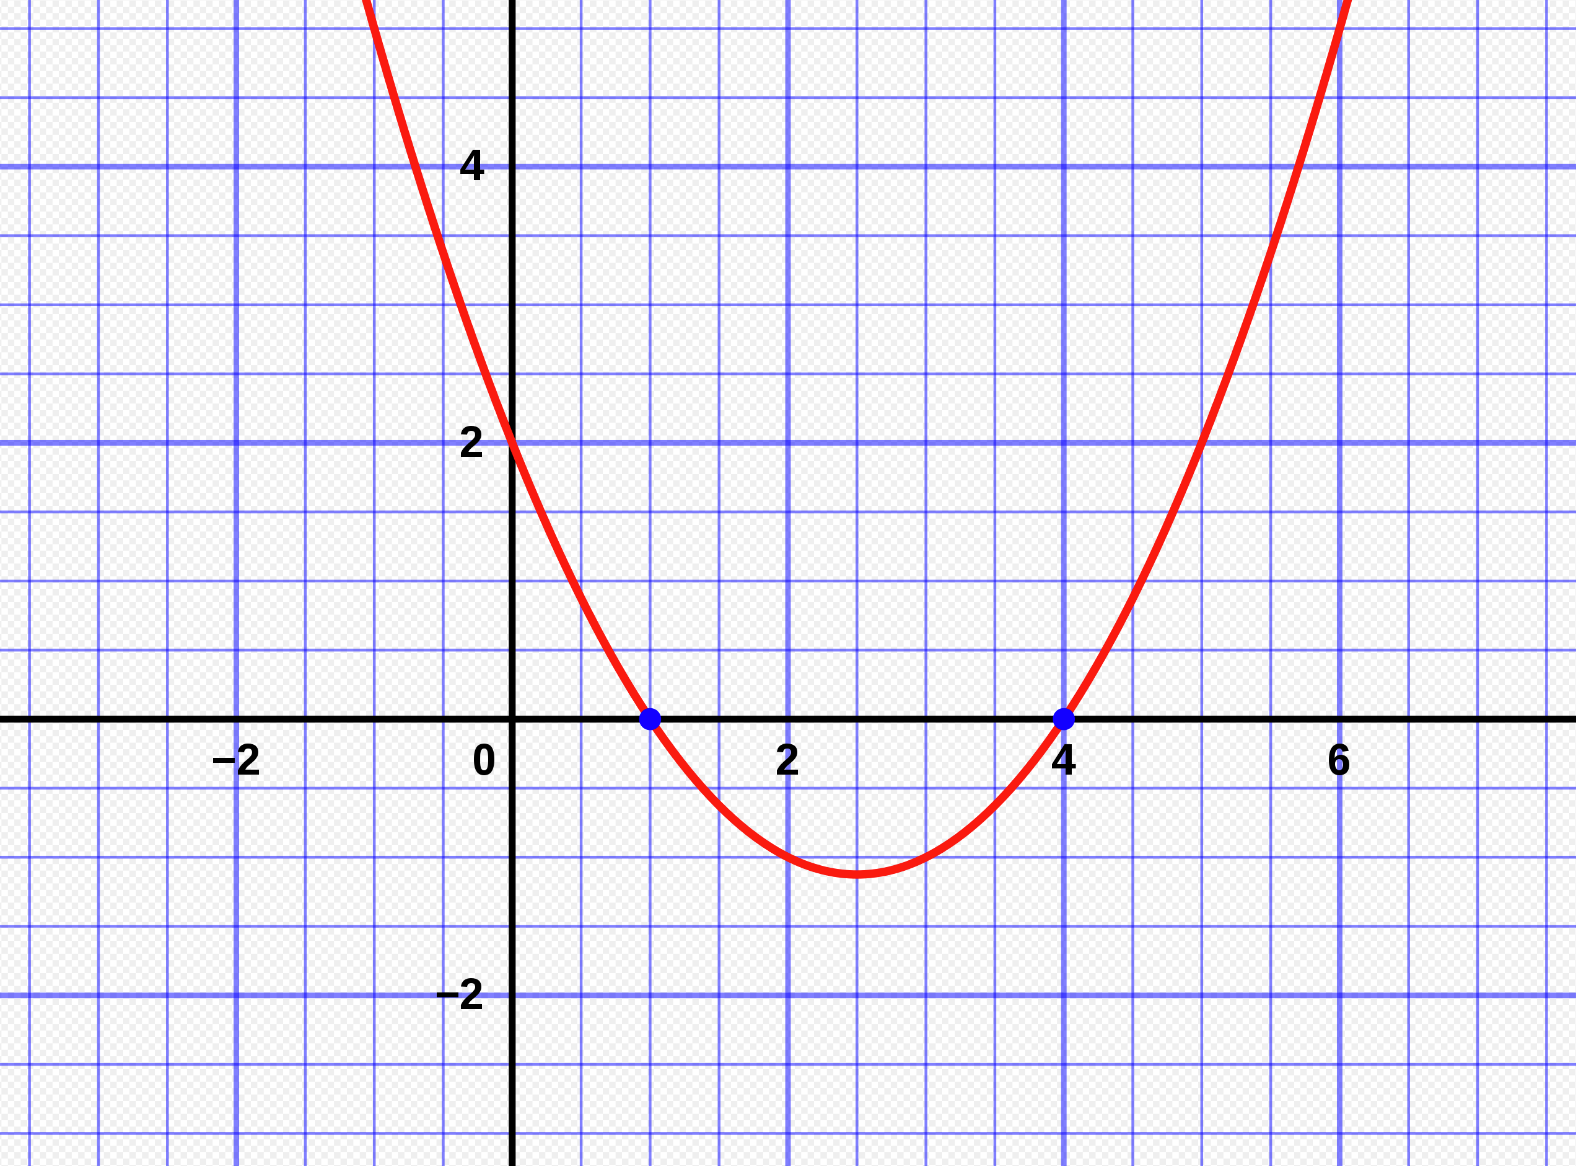
\includegraphics[scale=.15]{quad_equ.png} 

\begin{description}[labelindent=1cm]
	
	\item[\textbf{\underline{Overview:}}] \hfill \vspace{3mm}\\
	We are going to write a Python program to solve the quadratic equation. After finding the solution, the program will output the results to the screen.
	
	\item[\textbf{\underline{System Requirements:}}] \hfill \vspace{0mm}

\begin{itemize}
	\item {\bf Computer}: A computer is required to complete this tutorial. Any OS should work.
	\item {\bf Python:} You can use the online Python compiler ( \href{https://www.online-python.com/online_python_compiler}{Online Python Compiler}  ) or a Python system of your choice.
\end{itemize}

	\item[\textbf{\underline{Problem Statement:}}] \hfill \vspace{0mm}
	
	\begin{itemize}

		\item Given: The coefficients $a_2,a_1,a_0$ of a second order polynomial in the form shown
		\[y=a_2x^2+a_1x+a_0 \]
		
		\item Find: The solution or roots $x_1,x_2$ of the equation
		 
	\end{itemize}

\item[\textbf{\underline{Program Minimum Requirements:}}] \hfill \vspace{0mm}

The program should accomplish the following tasks. 


\begin{itemize}

	\item The coefficients $a_2,a_1,a_0$ should be stored as variables in the program.
	
	\item The roots $x_1, x_2$ should be calculated by the program.
	
	\item The calculated roots $x_1, x_2$ should be printed to the screen.

\end{itemize}	 
	Optional Advanced Features:
\begin{itemize}
	\item The inputs $a_2,a_1,a_0$ should be read from the user during program execution
		
	\item The program should handle equations with real and complex solutions without error. 
    
    \item The equation and solution should be plotted on an x-y graph.
    
\end{itemize}	
\newpage

\item[\textbf{\underline{Example Code:}}] \hfill \vspace{0mm}

	%\begin{minted}{cpp}
	\begin{lstlisting}

# Variables and Assignment - GSET - Summer 2023 
	
import numpy as np # include the numerical library

a2 = 10 # assign values to test code
a1 = 25  
a0 = 0   

x1=  # complete these lines
x2=  

print("The first root is", x1) // print the results
	
	\end{lstlisting}
	%\end{minted}
		


	\item[\textbf{\underline{Part 3 - Testing:}}] \hfill \vspace{0mm}
	\begin{enumerate}
	
		\item Complete the Python code to the solve the problem described. \\\\
		
		\item Test your code with different inputs. Is the answer correct? How do you know? Are there certain inputs that do not work? \\\\
		
		\item Save your code with the download button or use copy and paste. You can view and edit the code in any text editor. Also, save a copy of the program output for your tutorial summary. \\\\

	\end{enumerate}

\newpage
\item[\textbf{\underline{Solution Code:}}] \hfill \vspace{0mm}

\begin{lstlisting}

COMING SOON
	
\end{lstlisting}

\item[\textbf{\underline{Tutorial Complete:}}] \hfill \vspace{3mm}\\ 
	Congratulations, after completing {\it Tutorial 2 - Quadratic Equation}, you have begun learning to program in Python! You are now ready to start learning about more complex data structures and program flow. \\


\newpage
\item[\textbf{\underline{Tutorial Summary:}}] \hfill \vspace{3mm}\\ 
Write a brief summary of what you accomplished and what you struggled with the most. 

Include the following items in the summary:
\begin{itemize}

\item a copy of the output of your program
\item a description of what the program does and how to use it

\end{itemize}


\item[\textbf{\underline{Submission on Teams:}}] \hfill \vspace{3mm}\\ 
Use the appropriate assignment folder on ilearn to submit your program and summary. Submit the fol1owing items with your TNTech username in the filenames as shown below. \vspace{0mm}\\

\underline{Files for Tutorial 1 (TNTech Username : twhill21)}

\begin{itemize}

\item Tutorial Summary: \textbf{ twhill21\_summary2.txt}

\item Python Source Code: \textbf{ twhill21\_tutorial2.py}

\end{itemize}


\end{description}
\end{document}

